\part{Machine Learning in Production}

\chapter{Overview of the ML Lifecycle and Deployement}

\section{Steps of an ML Project}

\begin{enumerate}
    \item \textbf{Scoping — Define project:} Defining the project and deciding what to work on. What exactly do you want to achieve? What is the input ($X$) and what is the output ($Y$)?

    \item \textbf{Data — Define and establish a baseline:} Collect or acquire the data needed for your algorithm and establish a baseline for comparison.

    \item \textbf{Data — Label and organize data:} Label, classify, and organize the dataset properly.

    \item \textbf{Modeling — Select and train model:} Choose an appropriate model and train it on the data.

    \item \textbf{Modeling — Perform error analysis:} Analyze errors after training to understand model weaknesses.

    \item \textbf{Deployment — Deploy in production:} Write the necessary software and integrate the model into a production environment (often including non–ML code).

    \item \textbf{Deployment — Monitor and maintain system:} After deployment, maintain the system. This may include retraining the model with new data, feeding outputs back into the dataset, and updating the model until a better version can be deployed.
\end{enumerate}

\section{Key challenges}

\begin{itemize}
    \item Statistical issues
    \item Software engineering issues
\end{itemize}

\paragraph{Concept Drift / Data drift} - Loosely, this means what if you data changes after the system has been deployed?

\paragraph{} - Need to consider data may change over time.
Keep a test set of data which is recent.
Can test data on relatively recent data.
After the model has been deployed to production, need to consider if the data has changed again.
If the data has changed (different microphone for voice, camera for images)  this data can be different and then the performance of the model can degrade.
It is important to recognise how the data changed and if the learning algorithm needs to be changed as a result.
When data changes sometimes it is a gradual change.
Sometimes it changes suddenly which causes a shock to the system.

The term data drift is used when the input distribution X changes.

The term concept drift is used when the mapping X -> Y changes.

\subsection{Software Engineering Issues}

Considerations - Do you need a real time system or batch predictions.
This will affect how the software is built.
Consider computational resources of the cloud.
Consider low latency of the edge.
Need to consider the hardware resources available.
GPU/CPU and power of the machines etc.

Depending on the application, especially if it is a real-time application, latency and throughput are measures in queries per second amongst other software engineering metrics.
Other metrics.
Latency, throughput (how many queries per second do you need to handle given your computer resources)

Another is logging.
When building your system it may be useful to log as much of the data as possible for analysis and review as well as ot provide more data for retraining your learning algorithm in the future.

Another consideration is security and privacy.
Different applications will have different requirements and this will need to be considered in the design.
Consider regulatory environments and sensitive data.

\subsection{Considerations}

\begin{enumerate}
    \item Realtime or batch
    \item Cloud vs Edge / Browser
    \item Computer Resources (CPU / GPU / Memory)
    \item Latency, throughput (QPS)
    \item Logging
    \item Security and privacy
\end{enumerate}

\paragraph{Summary}

Deploying a system requires two broad sets of tasks.

There is writing the software to enable you to deploy the system in production.
There is what you need to do to monitor the system performance and to continue to maintain it, especially in the face of data drift and concept drift.
One thing to notice is that the practices for the very first deployments will be quit different compared to when you are updating or maintain a system that has already been previously deployed.


After an initial deployment the is more work that will need to be done.
Need to feed the data back into the model and potentially update the model even as the data / especaillly since the data will change.

\section{Deployment Patterns}

\subsection{Deployment use cases}

\begin{itemize}
    \item New product / capability - Offering a new product or capability that has not been previously offered.
    In this use case a common approach is to send a small amount of traffic and the gradually ramp it up.
    \item Automate / assist with manual task - Something already done by a person but now we would like to use a learning algorithm to automate and / or assist with the task.
    \item Replace a previous ML system - Already have a ML system but want to replace it with a better one.
\end{itemize}

Generally in these cases you will want a gradual ramp up with monitoring.

We want to avoid sending loads of traffic to a learning algorithm that has not been fully proven.
We send a small amount of data, and then we monitor it and then we ramp up the percentage or amount of traffic.

Another idea is a rollback.
If the algorithm isn't working at all or very badly we roll it back to the previous system, if there was an earlier system.

When you have people initially doing a task one common deployment pattern is to use shadow mode deployment.
This means that you will start by having machine learning algorithm shadow the numan inspector and run in parallel with the human inspector.
During this initial phase, the learning algorithms ouput is not used for any decisions.
Regardless of the machine learning algorithm, we go with the human judgement first.

The purpose of the shadow mode deployment is that it allows you to gather data of how the learning algorithm is performing and how that compares to human judgements.
By sampling the outputs, you can then verify if the learning algorithms predictions are accurate, and therefor use that to decide whether to maybe allow the learning algorithms to make some real decisions in the future.
When you already have a some system that is making good decisions, human inspectors or an older implementation of a learning algorithm, using shadow mode deployment can be a very effective way to let you verify the performance of a learning algorithm before letting it make any real decisions.

When you are ready to let a learning algorithm start making real decisions, a common deployment pattern is to use a canary deployment.
In a canary deployment, you would roll out to a small fractions, maybe 5\% or less of traffic initially and start letting the algorithm make the real decisions.
By running this on a small fraction of the traffic, hopefully if the algorithm makes any mistakes, it will only affect a small portion of the traffic.
This gives you more of an opportunity to monitor the system and ramp up the percentage of traffic it gets only gradually and only when you have greater confidence in its performance.
Ideally this style of deployment will allow you to spot problems early one, before there are maybe overly large consequences of what ever context the machine learning algorithm is being deployed in.

Another deployment pattern is blue-green deployment.
The old versions of the software is referred to as the blue version and the new version is called the green version (the new ML model being deployed.)
Eventually you would stop sending traffic to the blue one completely and switch over to the new one after initially sending some traffic to the blue version.

An advantage of blue-green deployment is that it is easy to rollback if something goes wrong.
Can reconfigure the router to direct traffic to the blue instance and spin up an instance of the blue version assuming that the blue version has been kept running.

Quite a lot of software will be needed to execute this ......

MLOps tools can help with implementing these deployment patterns, or it can be implemented yourself.
Rather than thinking about a system deployment as zero or one/ deploy or not deploy approach it from what is the appropriate degree of automation.
Partial automation with a human is a good design approach for applications where a learning algorithms performance isn't good enough for full automation.
This is a spectrum.

Consumer internet applications lend themselves to full automation.
Outside of this, human in the loop deployment may be the better approach.

\section{Monitoring}

The goal is here to make sure that a machine learning system is meeting your performance expectations.

The most common way to use a dashboard to rack how it is doing over time.
Depending on your application your dashboard may monitor different metrics.
Examples: Server load, diffraction of non-null outputs.
Example:  A speech recognition algorthm outputs null and thinks that the user didn't say anything.
If this was to change dramatically over time this would indicate that something is wrong.

A common example for structured data tasks.
Monitoring the fraction of missing input values.
If that changes, it may mean that something has changed about your data.

A goog approach when deciding what to monitor is to spend time with the team and brainstorm things that can possibly go wrong.
If something does go wrong and for all the things that could go wrong, brainstorm a few statistics or a few metrics that will detect that problem.
An approach is to start off with a lot of different metrics and monitor a relatively large set.
Gradually remove the ones that are not useful.

Some examples: Memory. compute, latency, throughput, server load.
Things that help you monitor the health of your software implementation fo the prefuction service or of other pieces of software around your learning algorithm.
Many MLOps tools with come with these metrics out of the box.

In addition to software metrics we could choose other metrics that help monitor the statistical health or the performance of the learning algorithm.

\subsection{Two types of statistical metricss}

One is input metrics.
Metrics that measure has you input distribution $$X$$ changed.
Number or percentage of missing values is a very common metrics when using structured data, some of which may have missing values.
-- Can brainstorm different metrics to see if your input distribution has changed



A second set of metrics that help you understand if your learning algorithm is performing well are output metrics.
How often does your system output null because it thinks there was no input when there was.
Could monitor the number of times that a user first tried to use the system before resorting to doing things manually.
Output metrics can help you figure out if either you learning algorithm output Y has changed in some way or can help you figure out you user behaviour has changed in some significant way.

Input and output metrics are application specific and need to be configured for the use-case.
Machine learning is highly iterative process as is deployment.

Once a deployment has been done and a number of dashboards have been setup this only the beginning of the iterative process.

In reality something may be deployed before finding out that something can go wrong and then new metrics can be introduced.

After you have chosen a set of metrics to monitor a common practice would be to set thresholds for alarms.

Many machine learning models will require retraining over time and maintenance just like software.
You can manually retrain where an engineer will retrain the model and performa error analysis on the model.
Or you could also put in a system in place where there is automatic retraining.
Today manual retraining is far more common than automatic retraining for many applications.


Developers are reluctant to let a learning algorithm be fully automatic in terms of deciding to retrain and push a new model to production.
There are some applications, especially in consumer internet where automatic retraining does happen.

\subsection{Summary}
By monitoring the system you can spot if there may be a problem that may cause you to go back to perform a deeper error analysis or that may cause you to go back to get more data which you can updated you model so as to maintain or improve you systems performance.
In that case you can be alerted that something needs to be fixed.

A typical scenario won't have s single machine learning model but multiple in a pipeline.

\section{Pipeline Monitoring}

Many AI systems are not just a single machine learning model running a prediction service but instead a pipeline that runs multiple steps.

A typical pipeline would be designed to not send any data to another system unless it has to.
Example would be sending voice to the cloud even though no one is talking.
This would waste resources/ bandwidth.

When you have two modules working together in a pipeline, changes in one can cause changes in the other module as well.

When you have machine learning pipelines these cascading effects can be very hard to keep a track of.
If there are sudden changes in the pipeline we would want to be alerted about it so we can update the system if we wanted to.

When building complex machine learning pipelines which can have machine learning components and non machine learning components throughout the pipeline, it may be useful to brainstorm metrics that can be used to detect changes.
Changes such as concept drift or data drift or bother and in multiple stages of the pipeline.

\subsection{Metrics to measure}

Monitor software metrics in the components of the pipeline or perhaps the pipeline as a whole.
Input metrica and potentially output metrics for each of the components in the pipeline.

By brainstorming metrics associated with individual components of the pipeline as well, this could help you spot a problems in components, and thereby alert you to changes in the data that may require you to take action to maintain the model.

Same metrics and principles at before but now we are looking at the whole pipeline.

Also need to consider how quickly the data changes.
The rate at which data changes is very problem dependent.

Some application wil have data that changes over years and moths and some may have data that changes in a matter of minutes.
On average user data changes very slowly.
User behaviour is generally quite slow to change but in the enterprise data can change quite fast.


\chapter{Modeling Challenges and Strategies}

\section{Modeling overview}
How to select and train the model
How to perform error analysis and use that to drive model improvements

Two modes of thought.
Model centric and data centric AI development.
A lot of emphasis on model centric.
Better to approach it from data centric view where you focus on not only the neural network architecture but on making sure you are feeding you feeding your algorithm high quality data.
That ultimately lets you be more efficient in getting your system to perform well.

Suggest that you don't engage in data centric AI development by collecting more data which time-consuming but use tools to help improve the data in the most efficient way.

\section{Key challenges}

AI system = Code(algorithm and/or model) + data

There are many projects where the algorithm or model is basically a solved problem.

A random model that is downloaded of GitHub is good enough, and it will be more efficient to spend a lot of your time improving the data because the data usually has been much more customised to your problem.

Diving into more detail, when building a machine learning system you may have an algorithm or model.
This would be your code and some data.
Its by training your algorithm on the data that you have your machine learning model that can make predictions.
Hyperparameters are an additional input to this process.

For many applications it is important to make sure you have a well tuned learning rate and regularization parameter and a few other thins?
Hyperparameters are important but the space of hyperparameters is relatively limited.

Model development is a highly iterative process.
You usually start off with some model and hyperparameters and data training model.
Then take the model to carry error analysis use that to help you decide how to improve the model or hyperparameters or the data.

Because machine learning is such an empirical process, being able to go through this loop many times very quickly, is key to improving performance.
One of the things that will help you improve performance too, is each time through the loop (see diagram) is being able to make good choices about how to modify the data or how to modify the model or how to modify the hyperparameters.

After you've done this enough times and achieved a good model, one last step that's often useful is to carry out a richer error analysis and have your system go through a final audit to make sure that it is working before you push it to a production deployment.

\subsection{Why is model development so hard?}

When building a model, there are three key milestones that most projects should aspire to accomplish.

First is you probably want to make sur you do well at least on the training set.
After you have done well on the training set, you have to ask if the algorithm does well on the development set or the holdout cross validation set and then also the test set.
If your algorithm isn't even doing well on the training set, the very unlikely to do well on the dev set or the test set

Think of step one as something you have to do first as a milestone on your way to wards achieving step two.
Then after you do well on the dev set or test set, you also have to make sure that you're learning algorithm does well according to the business metrics or according to project goals.

In the past a lot machine learning development was driven by the foal by doing well on the dev or test set.

For many problems having a high test set accuracy is not sufficient for achieving the goals of the project.
This has let to a lot of frustration and disagreements between the machine learning team and business teams which care more about the business metrics or some other goals of the project.

It is possible that low average test set error is not good enough for a project.

\section{Why low average error isn't good enough}

It is not enough to do well on the hold out test set.

In addition to concept drift and data drift there are some additional challenges we may have to address for production machine learning project.
First, a machine learning system may have low average test set error, but if its performance on  set of disproportionally important isn't  good enough, then the machine learning system will still not be acceptable for production deployment.

Two types of queries, informational / transactional queries and navigational queries where the use has a very clear intent and a very clear desire to go to something.

When a user has a very clear navigational intent, they will tend to be very unforgiving if a web search engine does anything other than return desired_thing as the number one ranked result.
A search engine that doesn't give the right results will quickly lose the trust of its users.

Navigational queries in this context are disproportionately important set of examples and if you have a learning algorithm that improves your average test set accuracy for web search but messages up just a small handful of navigational queries, that may not be acceptable for deployment.

The challenge, of course is that the average test set accuracy tends to weight all examples equally, whereas in web search.
Some queries are disproportionately important.


\subsection{Solutions}
One thing you could do is try to give these examples higher weight.
That could work for some applications, but just changing the weights of different examples doesn't always sort the entire problem.
Closely related to this is the question of performance on key slices of the data set.
-> very important in practice when obeying certain regulations and laws.
Even if a learning algorithm for load approval achieves high average test set accuracy, it would not be acceptable for production deployment if it exhibits an unacceptable level of bias or discrimination.

Generally there is a lot of discussion about fairness to individuals and it an important issue to address.
--> retailer may push products from large retailers etc.
Could be bad for business because you lose the small retailer since the recommender system only recommends the large retailers.

Need to be weary of "did well in the test set" but doesn't work for my application.
Doing well on just the test set is not good enough for machine learning applications.
Important to make sure that the application is actually meeting the businesses need rather than just passing some kind of test set.

\section{Establish a baseline}

When starting work on a machine learning project one of the most useful first steps is to establish a baseline.
Only after you have established a baseline level of performance that you can then have tools to efficiently improve on the baseline level.

Best practices for establishing a baseline are quite different depending on whether you're working on unstructured or structured data.
Unstructured data refers to data sets like images, audio and natural language.Unstructured data tends to be data that humans are very good at interpreting.

Because humans are good at unstructured data tasks measure human level performance of HLP is often a good way to establish a baseline if you are working on unstructured data.

Structured data.
Typically, tables, spreadsheets etc.
Not natural for humans.
Human level performance is a very bad baseline for structured data application.


Machine learning developments best practice is quire different, depending on whether you're working on an unstructured data or structured data problem.
Keeping in mind this difference, take a look at some ways to establish baselines for both of these types of problems.
HLP - Human Level Performance
Another way to establish a baseline is to do a literature search for state-of-the-art or look at open source results to see what others report they are to accomplish on this type of problem.

Using open source you may also consider coming out with a quick-and-dirty implementation.
--> Just a quick and dirt implementation could give you a sense of what may be possible

Finally, if you have a machine learning system running for your previous application then the performance of your previous system can also help you establish a baseline that you can then aspire to improve on.
What a baseline system or a baseline level of performance does it helps to indicate what might be possible.

In some cases such as it if you're using human level performance, especially in unstructured data problems this baseline can also give you a sens of what is the irreducible error or what is bayes error.
In other words, what is the best that anyone could possibly hope for in terms of performance on this problem.

By helping use to get a very rought sense of what might be possible it can help us be much more efficient in terms of  prioritising what to work one.

Can be in an awkward position to guarantee certain accuracies when the team hasn't even established a baseline.
In such a scenario you need push back  and ask for more time to establish a rough baseline level of performance before giving a more firm prediuctionm about how accurate the machine learning system can eventually get to be.
Establishing a baseline first will help set you and our team up better for long-term success.

\section{Tips for getting started}

Machine learning is an iterative process where you start with a model, data and hyperparameters, training model, carry out error analysis and then use that to drive further improvements.
After you have gone around the loop a few times, when you have a good enough model you might then carry out a final performance audit before taking to production.

Some suggestions for that for getting that first step.

%Very good advice
Always start with a quick literature search to see what's possible.
Can look at online courses, look at blogs, look at open source projects.

If your goal is to build a practical production system and not to do research, don't obsess about finding the latest greatest algorithm.

Pick something reasonable that lets you get started quickly.
If you can find an open source implementation that cna also help you establish a baseline more efficiently.

For many practical applications, a reasonable algorithm with good data will often do just fine and will in fact outperform a great algorithm with not so good data.

Don't obsess about taking the algorithm that was published "last week" that is the most cutting edge algorithm.
Instead, find something reasonable, find a good open source implementation and use that to get going quickly
Because being able to get started on this first step of this loop can make you more efficient in iterating through more times and that will help you get to good performance more quicjly.

Do i need to take into account deployment constraints such as compute constraints when picking a model?
Yes, they should be taken in to consideration.
Constraints such as computer constraints.

If the baseline is already established, and you're relatively confident that this project will work and does, you goal is to build and deploy a system.
But if you've not even established a baseline, of if you're nore suyet sure if this project will work and be worthy of deployment then no or maybe not necessarily.

If you are in a stage of the project where you first goal is just to establish a baseline and determine what is possible, if this project is even worth pursing it may be okay to ignore deployment constraints.
Find some open source implementation and try it out to see what might be possible, even if that open source implementation is so computationally intensive that you know you will never be able to deploy that.
- No harm in taking deployment constraints into account as well at this phase of the project.

It might also be okay if you don't and focus more efficiently establishing a baseline first.

Finally, when trying out the learning algorithm for the first time before running it on all you data, I would urge you to run a few quick sanity check for your code and your algorith.
- An example, overfit a very small bit of training data before spending hours, or sometimes even overnight, or days training the algorithm on a large data set.
- Maybe even tray to make sure you can fit one training example, especially if the output is a complex output.

Training for overfitting on a small example can allow you to find bugs and issues quickly before and this training is quite fast.
If an algorithm can do well on a 100 items it won't do well on a 10000/
This would be another useful sanity check for your code.

After you have trained a machine learning model, after you've trained your first model, one of the most important things is how do you carry out error analysis to help you decide how to improve the performance of your algorithm.

\section{Error analysis example}

The first time you train a learning algorithm.
you can almost guarantee that it won't work, not the first time out.
The heart of the machine leaning development process is error analysis.
If this can be done well you can tell what is the most efficient use of your time in terms of what you should do to improve your learning algorithms performance.

%Consider adding examples

Error analysis can be done manually in say a Jupyter notebook or tracking errors in a spreadsheet.
There are emerging MLOps tools that make this process easier for developers.
Error analysis is also an iterative process.

The goal of this process is to productively improve the algorithm.

\section{Prioritising what to work on}

To summarise when prioritising what to work on you might decide that the most important characteristic to work on, you might decide on the most important categories to work on based on how much room for improvement there is such as compared to human-level performance or according to some baseline comparison.

One fruitful approach is to consider adding data or improving the quality of the data for a category.
You can use "data augmentation" to get more data from a data category, that will be another way to improve your algorithms performance.

In machine learning we like to have more data but going out to collect more data generically, can be very time-consuming and expensive.
By carrying out an analysis like this, when you are then going through this iterative process of improving your learning algorithm, you can be much more focused in exactly what types of data you collect.

\section{Skewed datasets}

Datasets where the ratio of positive to negative examples is very far from 50/50 are called skewed datasets.

When hyou have a very skewed data set raw accuracy is not that useful of a metric to look at.
Its more useful to build something called a confusion matrix.

A confusion matrix is a matrix where on axis is labeled with the actual label.

SEE DIAGRAM. When you are building a confusion matrix you fill in with each of these four cells the total number of examples for each bucket.

True negatives
True positives
False positives
False negatives



Standard metrics to look at when comparing different models on skew datasets are precision and recall, where looking at these numbers helps you figure out all of the exampels.
Looking at these numbers helps you figure which truly positive examples did the algorithm manage to catch.

Some times you have a model with better recall and different model with better precision.

\[
    \begin{array}{c|c|c|}
        \multicolumn{1}{c}{} & \multicolumn{2}{c}{\textbf{Predicted}} \\
        \cline{2-3}
        \textbf{Actual} & \text{Positive} & \text{Negative} \\
        \cline{2-3}
        \text{Positive} & \text{TP} & \text{FN} \\
        \cline{2-3}
        \text{Negative} & \text{FP} & \text{TN} \\
        \cline{2-3}
    \end{array}
\]

\[
    \text{Precision} = \frac{{TP}}{{TP} + {FP}}
\]

\[
    \text{Recall} = \frac{{TP}}{{TP} + {FN}}
\]


\subsection{$F_{1}$ Score}

\[
    F_1 = \frac{2}{\frac{1}{{P}} + \frac{1}{{R}}}
\]

One intuition behind the $$F1$$ score is that you want an algorithm to do well on both precision and recall.
If it does worse on either precision oor recall, that's pretty bad.
$F_1$ score is a way of combining precision and recall that emphasises whichever of P or R of recall is worse.

In mathematics this is technically called the harmonic mean between precision an recall which is like talking an average but placing more emphasis on which is the lower number.

$$F_1$$ score is not the only metric.

\section{Performance Auditing}

Even when your algorithm is doing well on its $F_1$ score or some other appropriate metric, its often worth one last performance audit before you push it to production.
THis can sometimes save you from significant post deployment problems, let's take a look.

Here is framework you can for how you can double-check your systems for accuracy, fairness/bias and for other possible problems.

Step 1 is brainstorm the different ways the system might go wrong.
For example does the algorithm perform sufficiently well on different subsets of the data, such as individuals of a certain ethnicity or individuals of different genders?
Does the algorithm make certain errors such as false positives or false negatives, which you might worry about in skewed data sets.

How does it perform on rare and important classes?
These can be added to the ways that the system might go wrong.
For all the ways that you're worried about the system going wrong, you might establish metrics to assess the performance of your algorithm against these issues.

One very common design pattern you see, it that you will often be evaluating performance on slices of the data.
Rather than evaluating performance on your entire death set, you may be taking out all the individuals of a certain ethnicity or all individuals of a certain gender etc.

But to take a subset of the data, also called a slice of the data to analyse performance on those slices in order to check against these things that may be problems.
After establishing appropriate metrics, MLOps tools can also help trigger an automatic evaluation for each model to audit its performance.

\subsection{Exmaples}
TensorFlow has a package for TensorFlow model analysis or TFMA that computes detailed metrics on new machin learning models on different slices of data.
As a part of the process it is reccomended to get buy in from the business or the product owner that these are the most appropriate problems to worry about and a reasonable set of metrics to assess against these possible problems.
If you do find a problems it is good if it is found early since you can avoid pushing it to production.
You can then go back to update the system to address it before deploying a system that may cause problems downstream.

The way a system can go wrong is very problem dependent.
Different industries, different tasks will have very different standards.
In fact today, out standards in AI for what to consider an unacceptable level of bias of what is fair and what is not fair.

Those standards are still continuing to evolve in AI and in many specific industries.
Besst to do a search for you industry to see what is acceptable and to keep current with standards of fairness and all of our growing awareness for how to make out systems more fair and less biased.

Final tip - better to have a team of people that brainstorm what can go wrong for high stakes applications.
It is also good to get external advisors to help you brainstorms things to look out for, that can reduce the risk of you or your team being caught later by something that you hadn't though of.
Standards are evolving for what is considered fair and sufficiently unbiased in many industries.

It is a good topic for us to get ahead of and to proactively try to identify, measure against and solve problems rather than deploy a system to be surprised much later by some unexpected consequences.

It is hoped that with performance auditing you have higher confidence in your learning algorithm when you go out and push it to production.

\section{Data-centric AI development}

Say error analysis has caused you to decided to focus on improving your learning algorithms performance on data with a certain category or tag.

Model centric vs data centric approach to machine learning.

With a model centric approach to view of AI development, you would take the data you have and then try to work really hard to develop a model that does as well as possible on the data.
Because a lot of academic research in AI was driven by researchers downloading benchmark data set and trying to do well on that benchmark, most academic research on AI is mode-centric because the benchmark data set is a fixed quantity.
So in the model-centric view, you would hold the data fixed and iteratively improve the code or the model.
The is an important role to play in trying to come up with better models but there is a different view of AI development, which is more useful for many applications which a shift from model-centric to data-centric view.

In this view we think of the quality of data as paramount and you can use tools such as error analysis or data augmentation to systematically improve the data quality and for many applications if you data is good enough multiple models will do just fine.

In this view you can instead hold the code fixed and iteratively improve the data.

There is a role for model-centric development and there is a role for data-centric development.

In this approach we are asking the question "how do we make the data set even better"?

One of the most important ways to improve the quality of a data set is data augmentation.

\section{A useful picutre of data augmentation}

\begin{figure}[h!]
    \centering
    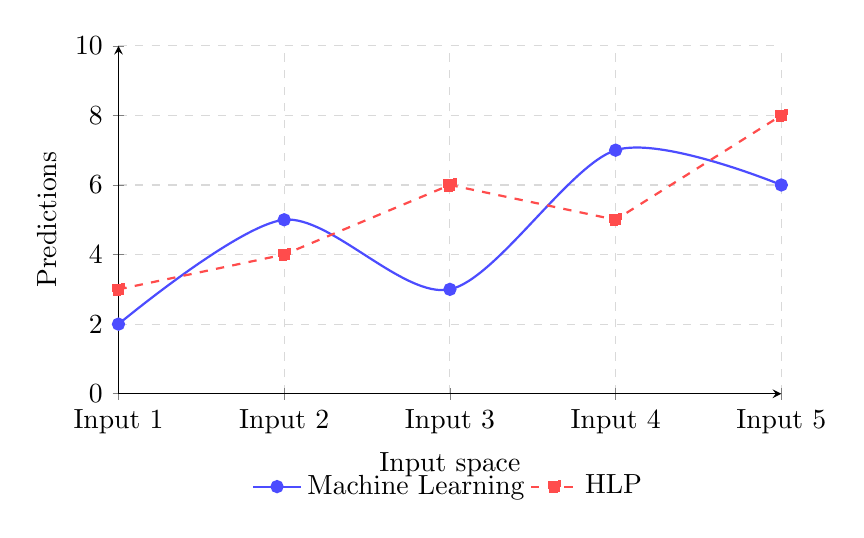
\begin{tikzpicture}
        \begin{axis}[
            width=10cm,
            height=6cm,
            xlabel={Input space},
            ylabel={Predictions},
            xtick={1,2,3,4,5},
            xticklabels={Input 1, Input 2, Input 3, Input 4, Input 5},
            ymin=0, ymax=10,
            grid=both,
            grid style={dashed, gray!30},
            axis lines=left,
            legend style={at={(0.5,-0.2)}, anchor=north, draw=none, fill=none},
            legend columns=-1
        ]

            % Machine Learning curve
            \addplot[
                thick,
                blue!70,
                smooth,
                mark=*,
                mark options={fill=blue!70}
            ] coordinates {
                (1,2)
                (2,5)
                (3,3)
                (4,7)
                (5,6)
            };
            \addlegendentry{Machine Learning}

            % HLP curve
            \addplot[
                thick,
                red!70,
                dashed,
                mark=square*,
                mark options={fill=red!70}
            ] coordinates {
                (1,3)
                (2,4)
                (3,6)
                (4,5)
                (5,8)
            };
            \addlegendentry{HLP}

        \end{axis}
    \end{tikzpicture}
    \caption{Comparison of predictions across inputs: Machine Learning vs. HLP.}
    \label{fig:predictions-curve}
\end{figure}

Collect more data to pull up the machine learning performance so that it is closer to human level performance.
By collect data for a particular input it could cause other parts to improve.

Use error analysis to measure how well the algorithm is performince.

\section{Data augmentation}

Create a lot of data efficiently which can be used for training.

The goal: Create realistic examples that
- THe algorithm does poorly on
- But humans (or other baseline) do well on

The goal of data augmentation is to create examples that you algorithm can learn from.
As a framework for doing that, thing about how you create realistic examples that algorithm does poorly on.
If the example does well in those examples, then there is less for it to learn from.
You want to the examples to still be ones that a human or maybe some other baseline does well on.

You want examples that are hard enough to challenge the algorithm but not so hard that they're impossible for any human or any algorithm to ever do well one.

Try to generate new examples using data augmentation that meets both criteria

One way to data augmentation is to generate an augmented data set and then train the learning algorithm and see if the algorithm does better on the dev set.
Fiddle around with the parameters for data augmentation and change the learning algorithm again and so on.
---- This turns out to be quite inefficient because every time you change you data augmentation parameters you need to train your new network or train your learning algorithm all over and this can take a long time.


Here is checklist for generating data.

1 - is it realistic? Is it realistic and like the data you want your algorithm to perform well on.
2 - Is the $X$ -> $Y$ mapping clear. In other words, can humanbs still recognise what was said?
3 - Three is the algorithm currently doing poorly on this new data. This helps you verify point one.

If you can generate data that meets all of these criteria, then that would give you a higher change then when you put this data in your training set and retrain the algorihtm.

Advanced / Fun technique for generating more examples.
Use GAN (Generative Adversarial Network).
- These techniques are overkill and there are faster and simpler techniques that work just fine without needing a GAN.

Model iteration - refers to iteratively training a model using error analysis and then tray to decide how to improve the model.

Taking a data centric approach to AI development.
- Sometimes it's useful to instead use a data iteration loop where you repeatedly take the data and the model, train your learning algorithm and do error analysis.
As you go through this loop, focus on how to add data or improve the quality of the data.

For many practical applications, taking a data iteration loop approach results in faster improvements to your learning algorithm performance depending on your problems.

When you're working on an unstructured data problem, data augmentation; ---- if you can create data that seems realistic, that humans can do quite well on, but the algorithm struggles on can be an efficient way to improve your learning algorithms performance.

If through data analysis you see that your learning algorithm does bad on certain types of data, then generating more data with this certain type could be an efficient way to improve your learning algorithms performance.

\section{Can adding data hurt?}

For a lot of machine learning problems, training sets, dev and test set distributions start at being reasonably similar.
If you're using data augmentation, you're adding to specific parts of the training set such as adding lots of data with specific traits.

You're training set may come from a very different distribution than then dev set and the test set.
Is this going to hurt your learning algorithms performance?
Usually the answer is no, with some unstructured data problems.

For unstructured data problems if:
- The model is large (low bias)
- The mapping x -> y is clear (e.g - given only the input x, humans can make accurate predictions)

Then adding data rarely hurts accuracy

This is important because adding data through data augmentation or collecting more of one type of data, can really change your input data distribution probability of $$X$$.

If your model is sufficiently large then it won't stop it from doing a good job on the data.

In contrast if your model was small then changing your input data distribution this way may cause it to spend too much of its resouces modelling the wrong thisgs.
This could hurt its performance on data which does not have this trait.
For large models this is not a problem.

Second Problem.
The mapping from X to Y is not clear, meaning given X the true label of Y is ambiguous.

Skewing the data set can hurt performance.

It is quite unusual for data augmentation or adding more data to hurt the performance of your learning algorithm,

So long as your model is big enough, maybe a neural network is big enough to learn from diverse set of data sources.

Data augmentation or collecting more data to improve the performance of your algorithm, even if it causes our training set distribution to become different from your dev set and test set distribution.

\section{Adding features}

For many structured data problems, it turns out that creating brand new training examples is difficult.
One thing you can do is take existing training examples and figure out if there are additional useful features you can add to it.
This doesn't need to be a binary feature.
It can be a soft feature like a percentage
Adding features can be a fruitful way to improve the performance of the algorithm.


There is a trend from collaborative filtering towards content based filter approaching.


Collaborative filtering recommended tings that a similar to the things similar users liked.

Content based filtering approach will ten to look at you as a person and look at a description.

The advantage of content based filtering is that even if there is a new product you can still make good recommendation.
Collaborative filtering would not be so effective since there are not other users for the new product.

This is sometimes called to cold start problem.
How do you recommend something that no one has every used before?
One way it to capture good features for this tings that you might want to recommend.
This is unlike collaborative filtering, which requires a bunch of people to look at the product and decide if they like it or not before it can decide whether a new users should be reccomended the same product.


Data iteration for structured data problems may look like this.
You start out with some model, train the model and then carry out error analysis.
Error analysis can be harder on structured data problems if there is no good baseline such as human level performance to compare to, and human level performance is hard for structured data because it is really difficult for people to recommend things even to each other.

Error analysis can discover good ideas for improvement, so can user feedback and so can benchmarking to competitors.

Features can be considered as a form of data which is why the form of data iteration can help you decide how to modify the features.
This can be an efficient way of improving your learning algorithms performance.

Before the rise of deep learning, the hope for deep learning was that you don't have to design features by hand any more.

Even with the rise of deep learning, if your dataset size isn't massive, there is still designing of features driven by error analysis that can be useful for applications.
The larger the data set, the more likely it is that a pure ene-to-end deep learning algorithm can work.

But for anyone other than the largest tech companies and even then for some applications, designing features, especially for structured data problems can still be a very important driver of performance improvements.

Maybe just don't do that for unstructured data nearly as much because learning algorithms are very good at learning features automatically for images, audio and for text maybe.
For structured data, its okay to go in and work on the features.

\section{Experiemnt Tracking}

Good to have as you work to make your machine learning algorithm more efficient.
Having a system to track your experiments can help you be more efficient in making the decisions on the data or the mode or hyperparameters to systemically improve you algorithm performance.


When you are tracking the experiments, meaning the models you have trained it is recommended to track the following.

One is to keep a track of what algorithm you are using and what version of code.
Keeping a record of this will make it much easier for you to go back and replicate an experiment you have run maybe two week ago and who's details you may not fully remember anymore.

Second keep a track of the data set you use

Third is track hyper parameters

Fourth save the results somewhere

This should include high level metrics such as accuracy or the $F_1$ score or other relevant metrics.

Tools to use for tacking experiments
- Text files  - doesn't scale well but is okay for small experiments
- Spreadsheets - scales a bit better
- Formal tracking tools
-> This space is growing.
Some tools Weights and biases, COmen, MLFlow, Sagemaker Studio, Landing AI

Things to look for in a tracking tool
- First does it give me all the information needed to replicate the results.
- In terms of replicability - does it give me all the information needed to replicate the results.
--- In terms of replicabilty, one thing to watch out for is if your learning algorithm pulls data off the internet.
---- Data off the internet can change, that can decrease replicabilty unless you're careful in how your system is implemented
---- Second tools that help you quickly understand the experimental results of a specific training run.
Ideally with useful summary metrics and maybe even a bit of an in depth analysis, can help you more quickly look at you more recent experiments.
------ Or even look at older experiments and remember what had happened..
--- Finally, some other features to consider are resource monitoring, how much CPU or GPU or memory resources did it use, tools to help you to visualise the trained model or even tools to help you with a more in depth error analysis.
Sometimes these are useful features of experieement tracking framewokrs.

Most importantly though you should have some kind of system, even if it is a spreadsheet or text file.
- Having that information is very useful for replicating results.

\section{From big data to good data}

Thoughts on shifting from big data to good data.

A lot of modern AI has grown up in large consumer internet companies with maybe a billion users and companies like that have a lot of data on their users.
If you have big data like that it means that you can boost the performance of your algorithm tremendously.
But both software consumer internet but equally important for many other industries

For many companies and other industries there just isn't a billion data points.
For those applications its important to focus on good data.
If you are able to ensure consistently high quality data in all phases in the machine learning project life cycle, that is key to making sure you have a high performance and reliable machine learning deployment.


What is mean by good data?
Good data covers the important cases, so you should have good coverage of different inputs $$X$$.
If you find about that you don't have good enough data, data augmentation can help you get more data and get more diverse inputs for X to give you that coverage.

Good data is also defined consistently with definition fo labels y that's unambiguous.
Good data also has timely feedback from production data.
--- Think monitoring systems to track concept drift and data drift.

Finally, you need a reasonable size data set.

\chapter{Data Definition and Base Line}

\section{Why is data definition hard?}

....for many practical applications, the way you prepare your data sets will have a huge impact on the success of machine learning project.

\section{More label ambiguity examples}

In the face of potentially very important and valuable prediction tasks like these, the ground truth can be ambiguous.
If you ask people to take their best guess at the ground truth label for tasks like these, giving labelling instructions that results in more consistent an less noisy and less random labels will improve the performance of your learning algorithm.
When defining data for you learning algorithm, here are some important questions.

First, what is the input X?
The right thing to do may not be to take this input X and just label it.
It may be to go to the factory and politely request improving the lighting because it is only with this better image quality that the labeler can then more easily see scratches like this and label them.
Sometimes it might be better to improve the quality of the sensor or improving the quality of input $$X$$.
That can be an important first set to ensuring your learning algorithm has a reasonable performance.

For structured data problems, defining which features to include can have a huge impact on your learning algorithms performance.

In addition to defining the input X, you also have to figure out what should be the target label $$Y$$.
A key question is how can we ensure labelers give consistent labels?

\section{Major types of data problems}

Best practices for organising data for one type can be quite different than the best practices for totally different types.

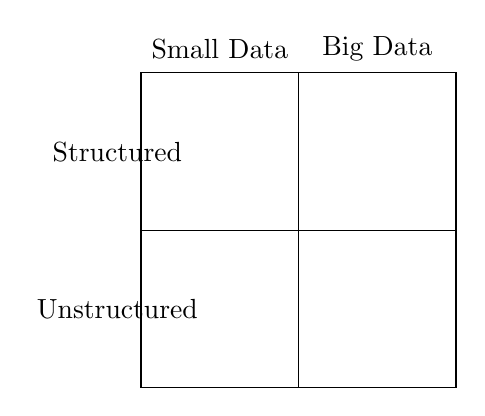
\begin{tikzpicture}
    % Draw 2x2 grid
    \draw (0,0) rectangle (4,4);
    \draw (2,0) -- (2,4);
    \draw (0,2) -- (4,2);

    % Labels
    \node at (1,4.3) {Small Data};
    \node at (3,4.3) {Big Data};
    \node at (-0.3,3) {Structured};
    \node at (-0.3,1) {Unstructured};
\end{tikzpicture}

Do you have a relatively small data set?
Do you have a large data set?
There is no precise definition but an arbitrary threshold of over 10,000 examples can be used.
This transition is a little but fuzzy and the transitions from small to big data sets is a gradual one.
The best practices if you have say 100 or 1000 examples smaller data sets is pretty different than we have a very large data set.
The reason I chose the number 10,000 is that's roughly the size beyond the size a human would do it.

Scale effects the best practices.

For a lot of unstructured problems, people can help you to label data and dat augmentation can also help.

In contrast for structured data problems, it can be harder to obtain more data and also harder to use data augmentation.


The second axis is the size of your data set.
When you have a relatively small data set, having clean labels is critical.
If you have 100 training examples, then if just one of the examples is mislabel, that's 1\% of you data set.

Because the data set is small enough for you or a small team to go through it efficiently, it may well be worth you while to go through that 100 examples and make sure each of those example sare labelled in a clean and consistent way.
Meaning according to a consistent labelling standard.

In contrast if you have a million data points, it can be harder and potentially impossible for a small machine learning team to manually go through every example.

Even when you have a lot of data, clean labels is better than non clean ones.
Because of the difficulty of having the machine learning and jointly go through evey example, the emphasis is on data processes.

In terms of how you collect and install the data the labelling instructions you may write for a large team of crowdsource labelers
And once you have executed som data process, such as ask a large team of labelers t o label a large set of audio clips, it can also be much harder to go back and change your mind and get everything relabeled.

%TODO insert 4x4 diagram

To summaries unstructured data problems.
You may not have a huge collection of unlabeled examples $$X$$.

For structured data problems, you can sometimes get more data by taking your unlabeled data x and asking humans to just label more of it.

This doesn't apply to every problem, but for the problems where you do have tons of unlabeled data, the can be very helpful and as we have already mentioned data augmentation can also be helpful.

For structured data problems it is usually harder to obtain more data because you only have so many users etc.
Human labelling on average is also harder although there are exceptions.

Small data vs Big data.
Small data
Clean labels are critical and teh data set may be small enough for you to manually look through the entire data set and fix any inconsistency in the labels.
 Can get all the labelers to talk to each other.

Big data.
- Emphasis is on the data process, you might have 100 or more labelers and ask them all to implement the same process.


This categorisation of small data vs big data and structured vs unstructured data is not only helpful for predicting if data processes generalise from one problem to another but also whether ot not machine learning idea is generalised from one to another.

If you are working on a problem from one of these four quadrants, then on average advice from some one who has worked on problems in the same quadrant will be more useful that advice from someone who has worked in a different quadrant.

Someone that has worked in the same quadrant as the problem I am trying to solve will usually be able to adapt more quickly to working on other problems in that quadrant.
There instincts and decision more similar within one quadrant that if you shift to totally different quadrant.

\section{Small data and label inconsistency}

in problems of a small dataset having clean and consistent labels is especially important.

Big data problems can have small data challenges as well.
- Problems with a large dataset but where there is a long tail of rare events in the input will have small data challenges too

\section{Improving label consistency}

- Have multiple labelers label the same examples
- Where there is disagreement, have the machine learning engineer, subject matter expert and / or labelers discuss definition of y to reach agreement.
- labelers believe that x doesn't contain enough information consider changing x
- iterate until it is hard to significantly increase agreement


Small data vs big data (unstructured data)
Small data
- usually small number of labelers
- can ask labelers to discuss specific labels
Big data
- get to consistent definition with a small group
- then send labelling instructions to labelers
- can consider having multiple labelers label every example and use voting or consensus labels to increase accuracy

\section{Human level performance}
Some machine learning tasks are trying to predict an inherently ambiguous output and human level performance can establish a useful baseline of performance as a reference.
Sometimes human level performance is misused.

In academia, HLP is ofter used as a respectable bench mark.
Beating human level performance can get a paper published etc.
--- In academia showing you can beat human level performance can get a paper published.

HLP can help establish a reasonable target

Mathematically proving performance on a test set is false logic.
Business need systems that do more than just doing well on average on test set accuracy.

The problem with beating Human Level performance as proof of machine learning superiority is multi fold.
The fact that most applications require more than just high average tested accuracy, one of the problems with this metric is that it sometimes gives a learning algorithm an unfair advantage when labeling instructions are inconsistent.

\section{Raising HLP}

- HLP in machine leaning had taken off partly because it helped people get papers published %no comment%
It has also been misused in setter where the goal is to build a valuable application, not just publish a paper.

When the ground truth is externally defined, there there are fewer problems with HLP when the ground truth really is some real ground truth.
But often ground truth is just another human label.

By raising HLP to 100\% it impossible for learning algorithm to beat HLP.
The benefit of this is you now have much cleaner, more consistent data and that ultimately will allow your learning algorithm to do better.

When your goal is to come up with a learning algorithm that actually generates accurate predictions rather just prove for some reason that you can bear HLP.
This approach of working to raise HLP is more useful.

Raising HLP
- When the label y comes from a human labeler HLP << 100\% may indicate ambiguous labelling instructions.
- Improving label consistency will raise HLP
- This makes  it harder for Machine learning to beat HLP. But the more consistent labels will raise ML performance, which ultimately likely to benefit the actual application performance.


HLP on structured data
- Structured data problems are less likely to invoke human labelers thus HLP is less frequently used

In the process of measuring HLP, you find that HLP is much less than perfect performance, much lower than 100\% then it is also worth asking yourself if that gap between HLP and 100\% accuracy may be due to inconsistent labeling instructions.
If that is the case then improving labelling consistency will both raise HLP but more importantly help you get cleaner and more consistent labels which will improve your learning algorithm's performance.

\section{Obtaining Data}

Need to consider how much time you should spend collecting data.
Machine learning is an iterative process where you need to pick a model, hyperparameters, have a data set and then training to carry out analusis.
Need to go around this loop multiple tiems to get to a good model.

Ideally you want to get into this iteration loop as quickly as possible.

After you have trained your initial model, carry out error analysis.
There will always be time to carry out more data.

This allows you to get into the iteration loop must more quickly and let the project make faster progress.
One exception to this guideline is if you have worked on this problem before and if from experience you know you need at least a certain training set size.
It might be okay to invest more effort up front to collect that much data

It terms of getting the data you need, one possible step is to take inventory of possible data sources.
--> can use crowd-sourcing  platform and pay people to read text.
--> can find a commercial supplier

Sit down and think through the tradeoffs when pick a method to collect data
Other factors include, regulatory and privacy constraints.

Having machine learning engineers do it is expensive but can help them build intuition about the data.
Beyond a certain point you may not want to spend all your time as a machine learning engineer labelling data and you might want to skip to a more scalable labelling process.

Depending on your application, there may also be different groups or sub groups of individuals that are going to more qualified to prove the labels.
More specialised tasks require an SME in order to provide accurate labels.
There are some applications where it is very difficult to get anyone to give good labels.

Tip: don't increase data by 10x at a time.

Genenerally want to avoid over investing in collecting data.


\section{Data pipelines}

Data pipelines, somtimes also called data cascades refers to when your data has multiple steps of processing before getting to the final output.

There are some practices that are relevant for some pipelines.

Given raw data, there is often some preprocessing or data cleaning before the data is fed to an learning algorithm that then tries to predict.
When you have scripts for data cleaning, one of the issues you run into is replicability when you take these systems into production deployment.

Meta-data

Useful for:
- Error analysis: Spotting unexpected effects
- Keeping track of data provenance

When you tak this system to production, you then have new data which has to be fed through a similar set of scripts because this data is going to be fed to the same machine learning algorithm.
Your machine learning algorithm on this data is what will run in  your product.
They key question is, if you preprocessing wad done with a bunch of scripts spread out on a bunch of different peoples computers and laptops, how do you replicate the scripts to make sure that the input distribution to you machine learning algorithm was the same for development data and the predictions data.


The amount of effort that you should invest to make sure that hte pre processing scripts are highly replicable can depend a little bit on the phase of the project.

When going the proof fo concept phase, the primary goal is just to decide if the application is workable and worth building and deploying
Advice to teams during the proof of concept phas is to focus on getting the prototype to work.
Its okay if some of the data preprocessing is manual.

If the project succeeds then you need to replicate all the preprocessing later.
- Take extensive notes, write extensive comments to increase the odds that you can replicate all this preprocessing later.
-- IImportant not to get bogged down in tons of process.
-- Just ensure replicability when the focus is really to just decide if the application is workable and it's worth taking to the next phase.
-- Once you have decided tha this project is worth taking to production then you know its going to be really important to replicate any preprocessing scripts.



In this phase, that's when I would use more sophisticated tools to make sure the entire data pipeline is replicable.
This is where the tools can be a bit more heavyweight.
- Tools like Tensorflow Transform, Apache Bean, Airflow and so on become very valuable.
- Many applications have more complex data pipelines.
- For those setting you also have to think about what metadata you want and perhaps also keep track and take care of data provenance and lineage.

\section{Meta-data, data provenance and lineage}

Data provenance and data lineage can be a big help.

%TODO add diagram

Arrows indicate flow of information or flow of computation.

To make sure that your system is maintainable, especially when a piece of data upstream ends up needing to be changes, it can be very helpful to keep track of data provenance as well as lineage.
Data provenance refers to where there data came from.
Lineage refers to the sequence of steps needed to get to the end if the pipeline.
At the very least, having extensive documentation could help you reconstruct data provenance and lineage, to build robust maintainable systems.. Not in the proof of concept stage but in the production stage.

There are more sophisticated tools to help you keep track of of what happens so that you can change part of the system and hopefully replicate the rest of the data pipeline without too much unnecessary complexity.
The tools for keeping track of data provenance and lineage are still immature in today's machine learning world.

Extensive documentation can help along with formal tools like TensorFlow.

To make life easier, bother manager data pipelines as well as for error analysis and riving machine learning development a key tip: make extensive use of meta data.
Metadata is data about data.

\section{Balanced train / dev / test / splits}

When your data set is small, having balanced training dev and tests sets can significantly improve your machine learning development process.

Balanced split where each of your training, dev and test has 30\% positive examples.
There is no need to worry about this effect when you have a large data set.
If you have a very large data set.
If you have a very large data set, a random split of data will very likely be representative, meaning that the percentage of positive examples will be quite close to your overall data set.
When you hava small data set with just 20 dev set examples and 20 test set examples, then explicitly making sure you have a balanced split can make your dev set and test set more reliable measures of your algorithms performance.
--> This is on of those techniques that can make a big different to you performance when you're working on a small data problem.
--> Don't to worry about the when you work on a very large data set.
When using a you have a smaller data set, consider using a balanced training dev test split in terms of how you setup your dataset.

\section{What is Scoping?}

\section{Scoping process}

When brainstorming projects to work on, get together with a business or product owner.
Often not an AI person but someone that understands a business or an applications and brainstorm with them what are their business or application problems.
At this stage we are trying to identify a business problem and not a AI problem.

Want to hear about business problems not AI problems and the provide an AI solution.
Separate the identification of the problem from the identification of the solution.
Having clear articulation on what the problem is helps us come up with better solutions.
This type of separation between problem and solution is something that will be heard of in design thinking as well.
After brainstorming a variety of different solutions, asses the desirability and the value of these different solutions.

Diligence.
Double checking if an AI solution is technically feasible and valuable.
After validating technical feasibility and the value or ROI return on investment on a project.
If it is promising we then flesh out the milestones for the project and finally budge for resources.

It is common for one problem to come up with multiple solutions

Worthwhile to engage in divergent thinking where you brainstorm a lot a possibilities to be followed by conversion thinking where you narrow it down to one or a small handful of the most promising projects to focus on.

\section{Dillgence on feasibility and value}

Is the project idea feasible before starting on the machine learning project.
How do you know if this thing can even be built?
One way to get a quick sense of feasibility is to use an external benchmark, such as the research literature or other forms of publications.
- or if a different company or even a competitor has managed to build a certain type of system before
- use some kind of external bench mark
To compliment an external bench mark or in the absence of an external bench mark there other ways to assess feasibility.

%TODO insert diagram

In addition to HLP the previous rate of progress on a project can be a reasonable rate of progress on a project.

Why use HLP to benchmark?
- People are very good on unstructured data tasks
Criteria - can a human, given the same data perform the task.
Importatnt that the human is only given the same information as what the machine would receive.

Sometimes the data is just not that predictable and you end up with a learning algorithm that does barely any better than random guessing.

%TODO diagram history of a project



\section{Dillegence on value}

Have technical and business teams try to agree on metrics that both are comfortable with

Ethical considerations
- Is this project creating net positive societal value?
- Is this project reasonable fair and free from bias?
- Have any ethical concerns been openly aired and debated?

\section{Milestones and resourcing}

Key specifications:
- ML metrics (accuracy, precision / recall, etc)
- Software metrics (latency, throughput, etc given compute resources)
- Business metrics (revenue, etc)
- Resources needed (data, personnel, help from other teams)
- Timeline

If you are unsure, consider benchmarking to other project, or building a POC (Proof of concept first)